\subsection{Implementation Details}\label{ssec:optim}
% \vspace{0.5\baselineskip}
\noindent
\textbf{Representation Model.} 
We employ the GET3D~\cite{gao2022get3d} architecture as object model $G$. Following StyleGAN~\cite{karras2019styleGAN,karras2020styleGAN2} embeddings $z_{T}$ and $z_{S}$ are mapped to intermediate style embeddings $\boldmath{w}_S$ and $\boldmath{w}_T$ in a learned $\boldmath{W}\text{-space}$, which we optimize over instead of $\boldmath{Z}\text{-space}$. Style embeddings condition a generator function that produces tri-planes representing object shapes as Signed Distance Fields (SDFs) and textures as texture fields. We deliberately \emph{train our generator on synthetic data only}, see experiments below. Differentiable marching tetrahedra previously introduced in DMTet~\cite{shen2021dmtet} extract a mesh representation and Images are rendered with a differentiable rasterizer~\cite{laine2020modular}.

\vspace{0.5\baselineskip}
\noindent
\textbf{Computational Cost.}
%
Each IR optimization step in our implementation takes $\sim$ 0.3 seconds per frame. The generation and gradient computation through the generator determines the computational cost of the method. However, we note that the rendering pipeline, contributing the majority of the computational cost of the generator, has not been performance-optimized and can be naively parallelized when implemented in lower-level GL+CUDA graphics primitives.

% \subsubsection{Computational Cost}
% %
% Each IR optimization step in our implementation takes $\sim$ 0.3 seconds per frame, with all six steps taking 1.8 seconds per frame, therefore the proposed approach does not work in real-time. The generation and gradient computation through the generator mainly determine the computational cost of the method, and we hope to see future work improve the computational cost of generative models. 

\begin{figure*}[t!]
	\centering
\resizebox{1.\linewidth}{!}{
	\renewcommand{\arraystretch}{0.5}
	\begin{tabular}{@{}c@{\hskip .05cm}c@{\hskip .05cm}c@{\hskip .05cm}c@{\hskip .05cm}c@{\hskip .05cm}c@{}}
		\centering
            &
		{\small Input $t_0$}&
		{\small Tracked $t_0$}&
		{\small Tracked $t_1$}&
		{\small Tracked $t_2$}&
		{\small Tracked $t_3$}\\

            \rotatebox[origin=c]{90}{{\footnotesize	Highway}}&
		\raisebox{-0.5\height}{\includegraphics[width=.32\columnwidth, trim={0cm 0cm 0cm 0cm},clip]{fig/waymo_main/scene1/waymo_s50_f45.png}}&
		\raisebox{-0.5\height}{\includegraphics[width=.32\columnwidth, trim={0cm 0cm 0cm 0cm},clip]{fig/waymo_main/scene1/waymo_s50_f45_bbox.png}}&
		\raisebox{-0.5\height}{\includegraphics[width=.32\columnwidth, trim={0cm 0cm 0cm 0cm},clip]{fig/waymo_main/scene1/waymo_s50_f46_bbox.png}}&
		\raisebox{-0.5\height}{\includegraphics[width=.32\columnwidth, trim={0cm 0cm 0cm 0cm},clip]{fig/waymo_main/scene1/waymo_s50_f47_bbox.png}}&
		\raisebox{-0.5\height}{\includegraphics[width=.32\columnwidth, trim={0cm 0cm 0cm 0cm},clip]{fig/waymo_main/scene1/waymo_s50_f48_bbox.png}}\\[1.3cm]

            \rotatebox[origin=c]{90}{{\footnotesize	Urban}}&
		\raisebox{-0.5\height}{\includegraphics[width=.32\columnwidth, trim={0cm 0cm 0cm 0cm},clip]{fig/waymo_main/scene2/waymo_44_38_gt.png}}&
		\raisebox{-0.5\height}{\includegraphics[width=.32\columnwidth, trim={0cm 0cm 0cm 0cm},clip]{fig/waymo_main/scene2/waymo_44_38_bbox.png}}&
		\raisebox{-0.5\height}{\includegraphics[width=.32\columnwidth, trim={0cm 0cm 0cm 0cm},clip]{fig/waymo_main/scene2/waymo_44_39_bbox.png}}&
		\raisebox{-0.5\height}{\includegraphics[width=.32\columnwidth, trim={0cm 0cm 0cm 0cm},clip]{fig/waymo_main/scene2/waymo_44_40_bbox.png}}&
		\raisebox{-0.5\height}{\includegraphics[width=.32\columnwidth, trim={0cm 0cm 0cm 0cm},clip]{fig/waymo_main/scene2/waymo_44_41_bbox.png}}\\%[0.0cm]
		
		
	\end{tabular}
	}
\vspace{-6pt}
\caption{Without changing the model or training on the dataset, our proposed method can generalize well to the Waymo Open Driving Dataset ~\cite{sun2020scalability}. Similar to Fig \ref{fig:nuScenes_results}, from left to right, we show (i) observed images from diverse scenes from the dataset at timestep $k=0$; (ii) an overlay of the closest generated object and predicted 3D bounding boxes at timestep $k=0, 1, 2 \text{ and } 3$. The color of the bounding boxes for each object corresponds to the predicted tracklet ID. Our method does not lose any tracks even on a different unseen dataset in diverse scenes, validating that the approach generalizes.}\label{fig:waymo_results}
\vspace*{-14pt}
\end{figure*}

% We first show the initial input frame at timestep k=0. Next to it, we present an overlay of the closest generated object and the refined bounding boxes. Reconstructions and bounding boxes for the next 3 frames are presented next to it. \todo{Description. Talk about color coding and that you don't lose any detections.}
\section{Experiments}\label{sec:exp}
In the following, we assess the proposed method. Having trained our generative scene model solely on simulated data~\cite{shapenet2015}, we test the generalization capabilities on the nuScenes \cite{caesar2020nuscenes} and Waymo~\cite{sun2020scalability} dataset -- both are unseen by the method. We analyze generative outputs of the test-time optimization and compare them against existing 3D multi-object trackers ~\cite{zhou2020CenterTrack, weng2020AB3DMOT, hu2021QD3DT,wang2023StreamPETR, yang2022qtrack} on camera-only data.

\subsection{Single-Shot Object Retrieval and Matching}
% \noindent
Although trained only on general object-centric synthetic data, ShapeNet~\cite{shapenet2015}, our method is capable of fitting a sample from the generative prior to observed objects in real datasets that match the vehicle type, color, and overall appearance closely, effectively making our method dataset-agnostic. 
We analyze the generations during optimization in the following.

\vspace{0.5\baselineskip}
\noindent
\textbf{Optimization.} Given an image observation and coarse detections, our method aims to find the best 3D representation, including pose and appearance, solely through inverse rendering. In Fig.~\ref{fig:optim} we analyze this iterative optimization process, following a scheduled optimization as described in Sec.~\ref{ssec:optim}. We observe that the object's color is inferred in only two steps. Further, we can observe that even though the initial pose is incorrect, rotation and translation are optimized jointly through inverse rendering together with the shape and scale of the objects, recovering from sub-optimal initial guesses. The shape representation close to the observed object is reconstructed in just 5 steps. 

% Prediction of reflectance and the integration and reconstruction of realistic environmental lighting is an exciting topic for future work.

\begin{table}[t!]
\centering
\caption{\textbf{Quantitative Evaluation for Camera-only Multi-Object Tracking}. Quantitative results on ``cars'' in the test split of the nuScenes tracking dataset~\cite{caesar2020nuscenes}. Our IR-based tracker outperforms AB3DMOT~\cite{weng2020AB3DMOT} on all metrics and CenterTrack~\cite{zhou2020CenterTrack} on accuracy. All three methods use the same detection backbone for fair comparison, while only CenterTrack requires end-to-end training on the dataset.
Additional results show on-par performance of our method with QD-3DT~\cite{hu2021QD3DT} trained on nuScenes \cite{caesar2020nuscenes}. QD-3DT trained on the Waymo Open Dataset (WOD) does not generalize to nuScenes and does not achieve competitive results. Only very recent transformer-based methods, such as PF-Track~\cite{pang2023PFtrack} and the metric learning approach of Q-Track~\cite{yang2022qtrack} achieve a higher score. However, these methods require end-to-end training on each dataset. ``CP'' denotes here the vision-only version of CenterPoint~\cite{zhou2019CenterPointVision} was used for object detection. \textbf{Bold} denotes best and \underline{underlined} second best for methods that did not train on the dataset or use the same detection backbone.}
\vspace*{-8pt}
\resizebox{\textwidth}{!}{
\begin{tabular}{l|l|cccc|c}
    \hline \hline
    \textbf{Training} & \textbf{Method} & \textbf{AMOTA} $\uparrow$ &	\textbf{AMOTP} (m) $\downarrow$ &	\textbf{Recall} $\uparrow$ & \textbf{MOTA} $\uparrow$ & \textbf{Modality} \\ 
    \textbf{Data Unseen} &  & &	& & & \\ 
        \hline
%%%%%%%%%%%%%%%% Table Content below
$\times$ & PF-Track~\cite{pang2023PFtrack} & 0.622 & 0.916 & 0.719 & 0.558 & Camera \\
$\times$ & QTrack ~\cite{yang2022qtrack} &  0.692 &  0.753 &  0.760 &  0.596 & Camera \\
$\times$ & QD-3DT ~\cite{hu2021QD3DT} & 0.425 &1.258 &  0.563 &  0.358 & Camera \\
\hline \hline
\textbf{\checkmark} & QD-3DT ~\cite{hu2021QD3DT} (trained on WOD) & 0.000 & 1.893 &  0.226 &  0.000 & Camera \\
$\times$ (CP) & CenterTrack~\cite{zhou2020CenterTrack} & 0.202 &1.195 &0.313 &0.134 & Camera \\
\textbf{\checkmark} (CP) & AB3DMOT ~\cite{weng2020AB3DMOT} & \underline{0.387} & \textbf{1.158} & \underline{0.506} & \underline{0.284} & Camera \\
\textbf{\checkmark} (CP) & Inverse Neural Rendering (ours) & \textbf{0.413} &  \underline{1.189} & \textbf{0.536} & \textbf{0.321} & Camera \\ % updated results as of Feb 15 2024

%%%%%%%%%%%%%%%% Table Content below
\hline \hline
\end{tabular}
}
\label{tab:nuScenes_results}
\vspace*{-14pt}
\end{table}

% results without hyper-param tuning
% Inverse Neural Rendering (ours) + CP~\cite{zhou2019CenterPointVision} & Camera& 0.248 &  1.140 & 0.485 & 0.193 & \checkmark \\

% best so far
% AMOTA	AMOTP	RECALL	MOTAR	GT	   MOTA	  MOTP	MT	 ML	  FAF	TP	   FP	 FN	    IDS	    FRAG	TID	    LGD
% 0.402	1.222	0.511	0.651	68518. 0.320  0.627	1281 2096 201.3	33691  11762 33509	1318	1307	1.29	2.30



%     \hline \hline
%     Method & AMOTA $\uparrow$ &	AMOTP (m) $\uparrow$ &	RECALL $\downarrow$ & MOTA $\uparrow$ &   IDS 	$\downarrow$ & No Dataset Training \\
%      &  &	 & & & & Training \\ \hline
% %%%%%%%%%%%%%%%% Table Content below
% PF-Track~\cite{pang2023PFtrack} & 0.622 & 0.916 & 0.719 & 0.558 &  99 &  $\times$ \\
% QTrack ~\cite{yang2022qtrack} &  0.692 &  0.753 &  0.760 &  0.596 & 617 &  $\times$ \\
% QD-3DT ~\cite{hu2021QD3DT}&  0.425 &1.258 &  0.563 &  0.358 &4293 &   $\times$ \\
% CenterTrack (Vision ~\cite{zhou2019CenterPointVision})  &0.202 &1.195 &0.313 &0.134 &2712 &  $\times$ \\
% \hline
% AB3DMOT + ~\cite{zhou2019CenterPointVision} & 0.387 & 1.158 & 0.506 & 0.284 &  1364 & \checkmark  \\
% InverseRenderTrack + ~\cite{zhou2019CenterPointVision} & 0.248 &  1.140 & 0.485 & 0.193 & 2153 & \checkmark \\
% %%%%%%%%%%%%%%%% Table Content below
% \hline \hline

 


% \begin{itemize}
%     \item Scene decomposition, including depth, segmentation, and object reconstruction on different scenes from KITTI and Waymo including Partial Occlusion, different levels of complexity (number of objects)
%     \item Tracking compared to "Quasi-Dense 3D tracking" with 3D boxes on a variety of Waymo and KITTI Scenes
%     \item Show a failure case of our method, demonstrating how easy it is to identify and explain/interpret.
%     \item Generalization to other domains, e.g. model trained on ShapeNet used for tracking on WAYMO and KITTI objects on a single object
%     \item Show the optimization process: 1. From a detection and sampled latent code to a refined object representation \& 2. From an object on one step in the tracking to a later step in the tracking process
% \end{itemize}

\subsection{Evaluation}\label{ssec:eval}
% \noindent
To provide a fair comparison of 3D multi-object tracking methods using monocular inputs, we compare against existing methods by running all our evaluations with the method reference code. We only evaluate methods, that consider past frames, but have no knowledge about future frames, which is a different task. While our method does not store the full history length of all images, we allow such memory techniques for other methods. We only consider purely mono-camera-based tracking methods.% following a two-staged detect and track approach. 
We note that, in contrast to our method, most \emph{baseline methods we compare to are finetuned on the respective training set}. For all two-stage detect-and-track methods, we use CenterPoint~\cite{yin2021center} as the detection method. We compare to CenterTrack~\cite{zhou2020CenterTrack} as an established learning-based baseline, and present results of the very recent PFTrack~\cite{pang2023PFtrack}, a transformer-based tracking method, Qtrack~\cite{yang2022qtrack} as a metric learning method, and QD-3DT~\cite{hu2021QD3DT} as an LSTM-based state tracker combined with image feature matching. 
Of all learning-based methods, only CenterTrack~\cite{zhou2020CenterTrack} allows us to evaluate tracking performance with identical detections. Finally, we compare to AB3DMOT ~\cite{weng2020AB3DMOT} that builds on an arbitrary 3D detection algorithm and combines it with a modified Kalman filter to track the state of each object. AB3DMOT~\cite{weng2020AB3DMOT} and the proposed method are the only methods that are data-agnostic in the sense that they have not seen the training dataset. For a fair evaluation of these generalization capabilities in learning-based methods, we include another version of QD-3DT solely trained on the Waymo Open Dataset~\cite{sun2020scalability} and evaluate on nuScenes~\cite{caesar2020nuscenes}.  We discuss the findings in the following.
%, we achieve the highest scores in all metrics, see Tab.~\ref{tab:matching_ablations}, conducted on the validation split. 

%This method is the most similar to our method in the sense that the Kalman filter parameters are not tuned for each dataset.


\begin{figure*}[t!]
	% \vspace{-12pt}
	% \renewcommand{\arraystretch}{0.5}
\centering
\resizebox{1.\linewidth}{!}{%
\begin{tabular}{@{}c@{\hskip .1cm}c@{\hskip .1cm}c@{\hskip .1cm}c@{\hskip .1cm}c@{}}

{Input Frame} & {Initial Guess} & {Texture Fitting} & {Object Pose Fitting} & {Shape Fitting} \\
	    
\includegraphics[width=.25\columnwidth, trim={0cm 0cm 0cm 0cm},clip]{fig/optim/optim_input.png}&
\includegraphics[width=.25\columnwidth, trim={0cm 0cm 0cm 0cm},clip]{fig/optim/init_im_w_bbox.png}&
\includegraphics[width=.25\columnwidth, trim={0cm 0cm 0cm 0cm},clip]{fig/optim/texture_im_w_bbox.png}&
\includegraphics[width=.25\columnwidth, trim={0cm 0cm 0cm 0cm},clip]{fig/optim/pose_im_pil.png}&
\includegraphics[width=.25\columnwidth, trim={0cm 0cm 0cm 0cm},clip]{fig/optim/final_im_w_bbox.png}\\
& \multicolumn{4}{r}{\textit{Input frame is faded for visibility.}} \\
\end{tabular}}
\vspace*{-6pt} 
\caption{\textbf{Optimization Process.} From left to right, we show (i) the observed image, (ii) the rendering predicted by the initial starting point latent embeddings, 
(iii) the predicted rendered objects after the texture code is optimized (iv) the predicted rendered objects after the translation, scale, and rotation are optimized, and (v) the predicted rendered objects after the shape latent code is optimized. The ground truth images are faded to show our rendered objects clearly. Our method is capable of refining the predicted texture, pose, and shape over several optimization steps, even if initialized with poses or appearance far from the target -- all corrected through inverse rendering.} 
\label{fig:optim}
\vspace*{-16pt}
\end{figure*}


\vspace{0.5\baselineskip}
\noindent
\textbf{Validation on nuScenes.} Tab.~\ref{tab:nuScenes_results} reports quantitative results on the test split of the nuScenes tracking dataset~\cite{caesar2020nuscenes} on the car object class for all six cameras. We list results for the multi-object tracking accuracy (MOTA)~\cite{bernardin2006MOTA} metric, the AMOTA~\cite{weng2020AB3DMOT} metric, average multi-object tracking precision (AMOTP)~\cite{weng2020AB3DMOT} and recall of all methods. First, we evaluate a version of QD-3DT~\cite{hu2021QD3DT} that has been trained on the Waymo Open Dataset~\cite{sun2020scalability} (WOD) but tested on nuScenes. This experiment is reported in row four of Tab.~\ref{tab:nuScenes_results} and confirms that recent end-to-end detection and tracking methods do not perform well on unseen data (see qualitative results in the Supplementary Material). Moreover, perhaps surprisingly, even when using use the same vision-only detection backbone as in our approach, the established end-to-end trained baseline CenterTrack~\cite{zhou2020CenterTrack}, which has seen the dataset, performs worse than our method.
Our IR-based method outperforms the general tracker AB3DMOT~\cite{weng2020AB3DMOT}. % in all metrics.
When other methods are given access to the dataset, recent learning-based methods such as the end-to-end LSTM-based method QD-3DT~\cite{hu2021QD3DT} perform on par.  Only the most recent transformer-based methods such as PF-Track~\cite{pang2023PFtrack} and the QTrack~\cite{yang2022qtrack}, which employ a quality-based association model on a large set of learned metrics, such as heat maps and depth, achieve higher scores. Note again, that these methods, in contrast to the proposed method, have been trained on this dataset and cannot be evaluated independently of their detector performance.

We visualize the rendered objects predicted by our tracking method in Fig.~\ref{fig:nuScenes_results}. We show an observed image from a single camera at time step $k = 0$, followed by rendered objects overlaid over the observed image at time step $k = 0, 1, 2 \text{ and } 3$ along with their respective bounding boxes, with color-coded tracklets. We see that our method does not lose any tracks in challenging scenarios in diverse scenes shown here, from dense urban areas to suburban traffic crossings, and handles occlusions and clutter effectively. By visualizing the rendered objects as well as analyzing the loss values, our method allows us to reason about and explain success and failure cases effectively, enabling explainable 3D object tracking. The rendered output images provide interpretable inference results that explain successful or failed matching due to shadows, appearance, shape, or pose. For example, the blue car in the IR inference in Fig.~\ref{fig:BEV3D_fig} top row was incorrectly matched due to an appearance mismatch in a shadow region. A rendering model including ambient illumination may resolve this ambiguity, see further discussion in the Supplementary Material.

\vspace{0.5\baselineskip}
\noindent
\textbf{Interpretation.} Fig~\ref{fig:BEV3D_fig} shows the inverse rendered scene graphs in isolation and birds-eye-view tracking outputs on a layout level. Our method accurately recovers the object pose, instance type, appearance, and scale. As such, our approach directly outputs a 3D model of the full scene, i.e., layout and object instances, along with the temporal history of the scene recovered through tracking -- a rich scene representation that can be directly ingested by downstream planning and control tasks, or simulation methods to train downstream tasks. As such, the method also allows us to reason about the scene by leveraging the 3D information provided by our predicted 3D representations. The 3D locations, object orientations, and sizes recovered from such visualizations can not only enable us to explain the predictions of our object tracking method, especially in the presence of occlusions or ID switches but also be used in other downstream tasks that require rich 3D understanding, such as planning. 

\begin{figure}[t!]
	% \vspace{-12pt}
	 \renewcommand{\arraystretch}{0.4}
	\centering
	\resizebox{1\columnwidth}{!}{%
	\begin{tabular}{@{}c@{\hskip .1cm}c@{\hskip .1cm}c@{\hskip .1cm}c@{\hskip .1cm}c@{\hskip .1cm}c@{}}
	    \multicolumn{2}{c}{\large (i) Input Frame} & \multicolumn{2}{c}{\large (ii) INR 3D Generation} & \multicolumn{2}{c}{\large (iii) INR BEV Layout} \\
    	\includegraphics[width=.31\columnwidth, trim={0cm 0cm 0cm 0cm},clip]{fig/BEV_and_3D/scene1/nusc_sc_3_cam_5_f9_gt.png}&
         	\includegraphics[width=.31\columnwidth, trim={26cm 6.7cm 12.5cm 15cm},clip]{fig/BEV_and_3D/scene2/gt_img.png}&
    	\includegraphics[width=.31\columnwidth, trim={0cm 0cm 0cm 0cm},clip]{fig/BEV_and_3D/scene1/sc_3_cam5_f9_rgb_out.png}&
         	\includegraphics[width=.31\columnwidth, trim={26cm 6.7cm 12.5cm 15cm},clip]{fig/BEV_and_3D/scene2/rgb_out.png}&
    	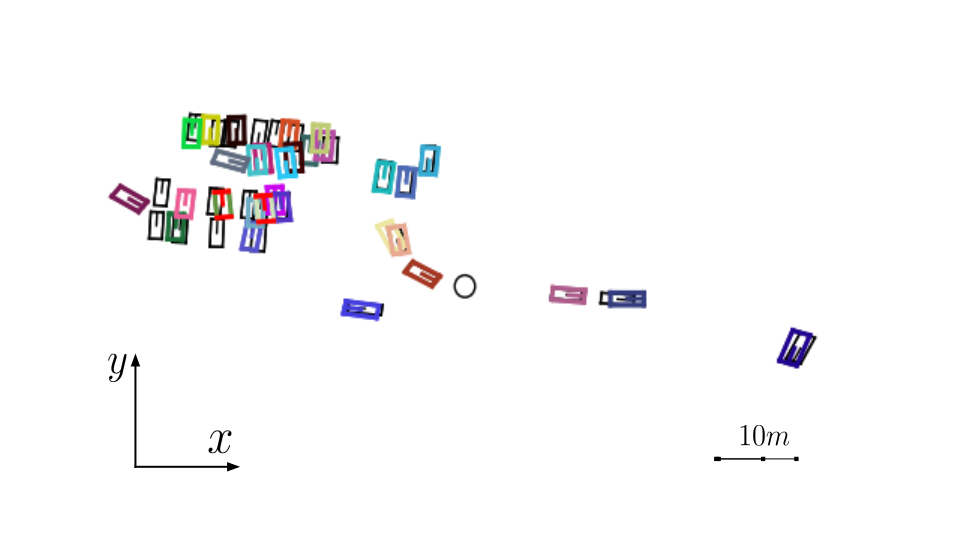
\includegraphics[width=.31\columnwidth, trim={2.1cm 2cm 1.9cm 2cm},clip]{fig/BEV_and_3D/BEV_axis_1.png}&
     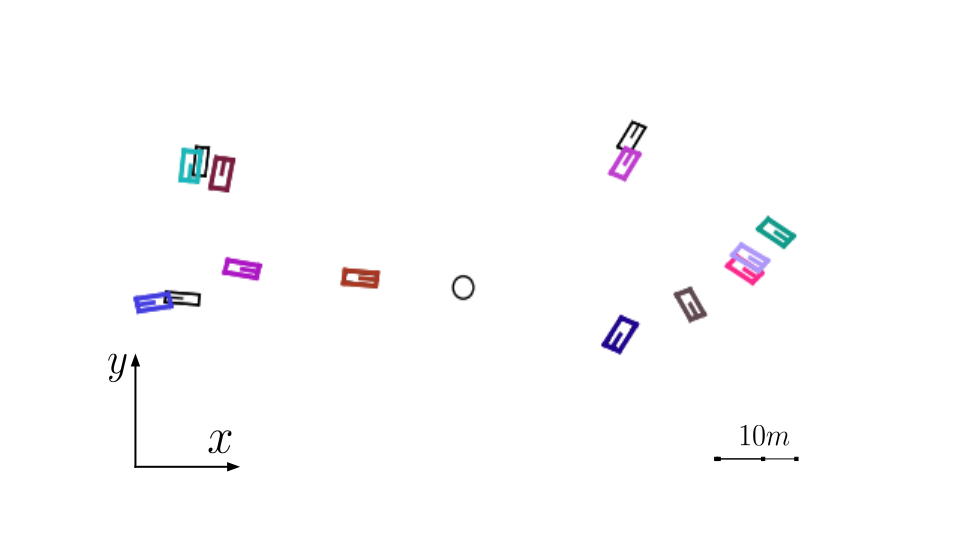
\includegraphics[width=.31\columnwidth, trim={2.1cm 2cm 1.9cm 2cm},clip]{fig/BEV_and_3D/BEV_axis_2.png}\\
     \textbf{\large (a)} & \textbf{\large (b)} & \textbf{\large (a)} & \textbf{\large (b)} & \textbf{\large (a)} & \textbf{\large (b)} \\
    \end{tabular}}
    \vspace*{-6pt}
\caption{\textbf{Layout Generation Through Inverse Rendering.} From left to right, we show (i) observed image from a single camera for two scenes (a, b), (ii) test-time optimized inverse rendered (IR) objects of class ``car'', and (iii) Bird's Eye View (BEV) layout of the scene. In the BEV layout, black boxes represent ground truth, and the colored boxes represent our predicted BEV boxes. The bottom shows a zoomed-in region at a 60 m distance (see BEV layout). Even in this setting, our method accurately recovers the 3D location, orientation, size, coarse appearance, and shape of the objects.} 
\label{fig:BEV3D_fig}
\vspace*{-16pt}
\end{figure}


\vspace{0.5\baselineskip}
\noindent
\textbf{Validation on Waymo.}
Next, we provide qualitative results from the 3D tracking on the validation set of WOD~\cite{sun2020scalability} in Fig.~\ref{fig:waymo_results}. The \emph{only public results} on the provided test set are presented in QD-3DT~\cite{hu2021QD3DT}, which may indicate it fails on this dataset. While the size of the dataset and its variety is of high interest for all autonomous driving tasks, Hu et al.~\cite{hu2021QD3DT} conclude that vision-only test set evaluation is not representative of a test set developed for surround view lidar data on partial unobserved camera images only. As such, we provide here qualitative results in Fig.~\ref{fig:waymo_results}, which validate that the method achieves tracking of similar quality on all datasets, providing a generalizing tracking approach. We show that our method does not lose tracks on Waymo scenes in diverse conditions.

% \begin{table}[t]
\centering
\resizebox{0.9\linewidth}{!}{
\begin{tabular}{l|lll}
    \hline
    \hline
    Method & AMOTA $\uparrow$ & Recall $\uparrow$  & MOTA$\uparrow$  \\
    \hline
    No Schedule & 0.102 & 0.224 & 0.110  \\
    \hline
    $\mathcal{L}_{RGB}$ - Eq.~\ref{eq:loss_mse} & N/A  & N/A & N/A  \\
    $\mathcal{L}_{perceptual}$ - Eq.~\ref{eq:loss_lpips} & 0.100 & 0.251 & 0.101 \\
    $\mathcal{L}_{IR}$ - Eq.\ref{eq:loss_mse_lpips}  & 0.103 & 0.236   & 0.112 \\
    $\mathcal{L}_{IR}$ \& $\mathcal{L}_{embed}$ - Eq.\ref{eq:regularize}  & \textbf{0.112} & \textbf{0.264 } & \textbf{0.113} \\
\hline
\hline
\end{tabular}
}
\caption{\todo{(a) Make split figure} \textbf{Ablation Experiments on Optimization Schedule and Loss Components.} Ablations were run on a small subset of the nuScenes~\cite{caesar2020nuscenes} validation set.  $\mathcal{L}_{RGB}$ fails due to the optimizer fitting objects to the background instead, increasing the size of each object resulting in out of memory.}
\label{tab:optim_ablations}
\end{table}

% \begin{table}[ht!]
\centering
\resizebox{0.95\linewidth}{!}{
\begin{tabular}{l|lll}
\hline
\hline
    Method (split)            & AMOTA $\uparrow$  & Recall $\uparrow$ & MOTA $\uparrow$   \\
    \hline
    AB3DMOT + CP (test) & 0.387             & 0.506             & 0.284             \\
    \hline
    Best Hyper-parameters (test)       & \textbf{0.402}    & \textbf{0.511}    & \textbf{0.320        }     \\
    \hline
    $w_{iou} = 1.4 $ (validation)   & 0.403             & 0.540             & 0.322               \\
    $w_{center} = 0.9$ (validation) & 0.417             & 0.514             & 0.332             \\
    $w_{embedd} = 0.4$ (validation) & 0.418             & 0.558             & 0.332             \\
    $\tau_{det} = 0.4$ (validation) & 0.397             & 0.567            & 0.326             \\
\hline
\hline
\end{tabular}
}
\caption{\textbf{Optimized Matching and Detection Confidence.} Parameters were optimized on the nuScenes \cite{caesar2020nuscenes} validation set. On the test split our best setting with $w_{iou} = 1.4$, $w_{center} = 0.9$, $w_{embbed} = 0.4$, $\tau_{det} = 0.4$ surpasses the performance of AB3DMOT \cite{weng2020AB3DMOT}, the only baseline not trained on the dataset. Results for other baselines are given in Tab. \ref{tab:nuScenes_results}. \todo{rewrite} }\label{tab:matching_ablations}
\vspace{-12pt}
\end{table}
% \begin{table}[t]
\centering
\resizebox{0.9\linewidth}{!}{
\begin{tabular}{l|lll}
    \hline
    \hline
    Method & AMOTA $\uparrow$ & Recall $\uparrow$  & MOTA$\uparrow$  \\
    \hline
    No Schedule & 0.102 & 0.224 & 0.110  \\
    \hline
    $\mathcal{L}_{RGB}$ - Eq.~\ref{eq:loss_mse} & N/A  & N/A & N/A  \\
    $\mathcal{L}_{perceptual}$ - Eq.~\ref{eq:loss_lpips} & 0.100 & 0.251 & 0.101 \\
    $\mathcal{L}_{IR}$ - Eq.\ref{eq:loss_mse_lpips}  & 0.103 & 0.236   & 0.112 \\
    $\mathcal{L}_{IR}$ \& $\mathcal{L}_{embed}$ - Eq.\ref{eq:regularize}  & \textbf{0.112} & \textbf{0.264 } & \textbf{0.113} \\
\hline
\hline
\end{tabular}
}
\caption{\todo{(a) Make split figure} \textbf{Ablation Experiments on Optimization Schedule and Loss Components.} Ablations were run on a small subset of the nuScenes~\cite{caesar2020nuscenes} validation set.  $\mathcal{L}_{RGB}$ fails due to the optimizer fitting objects to the background instead, increasing the size of each object resulting in out of memory.}
\label{tab:optim_ablations}
\end{table}

\begin{table}[t]
% 1. Table
\caption{\textbf{Ablation Experiments}}
\vspace*{-18pt}
\begin{subtable}[t]{0.485\linewidth}
\centering
\caption{\textbf{Optimization Schedule and Loss Components.} Ablations were run on a small subset of the nuScenes~\cite{caesar2020nuscenes} validation set.  $\mathcal{L}_{RGB}$ fails due to the optimizer fitting objects to the background instead, increasing the size of each object resulting in out of memory.}
% \vspace*{-8pt}
\resizebox{0.98\textwidth}{!}{
\begin{tabular}{l|lll}
    \hline
    \hline
    Method & AMOTA $\uparrow$ & Recall $\uparrow$  & MOTA$\uparrow$  \\
    \hline
    $\mathcal{L}_{IR}$ \& $\mathcal{L}_{embed}$ - Eq.\ref{eq:regularize}  & \textbf{0.112} & \textbf{0.264 } & \textbf{0.113} \\
    $\mathcal{L}_{IR}$ - Eq.\ref{eq:loss_mse_lpips}  & 0.103 & 0.236   & 0.112 \\
    $\mathcal{L}_{perceptual}$ - Eq.~\ref{eq:loss_lpips} & 0.100 & 0.251 & 0.101 \\
    $\mathcal{L}_{RGB}$ - Eq.~\ref{eq:loss_mse} & N/A  & N/A & N/A  \\
    \hline
    \underline{No Schedule} & 0.102 & 0.224 & 0.110  \\
\hline
\hline
\end{tabular}
}
\label{tab:optim_ablations}
\end{subtable}
\hfill
% 2. Table
\begin{subtable}[t]{0.485\linewidth}
\centering
\caption{\textbf{Effect of Optimization Schedule.} (a) observed image, (b) optimized generations using the proposed schedule in Sec.~\ref{sec:method}, (c) optimized generations using no schedule. This supports the quantitative to the left.}
\vspace*{-8pt}
\renewcommand{\arraystretch}{0.4}
\centering
\resizebox{1\columnwidth}{!}{
\begin{tabular}{@{}c@{\hskip .1cm}c@{\hskip .1cm}c@{}}

    \multicolumn{1}{c}{(a) Input Frame} &
    \multicolumn{1}{c}{(b) Full (ours)} & 
    \multicolumn{1}{c}{(c) \underline{No Schedule}} \\
    
    \includegraphics[width=.5\columnwidth, trim={0cm 0cm 0cm 0cm},clip]{fig/rebuttal_optimization/gt/11_102_gt.png}&
    \includegraphics[width=.5\columnwidth, trim={0cm 0cm 0cm 0cm},clip]{fig/rebuttal_optimization/sched/11_102_sched.png}&
    \includegraphics[width=.5\columnwidth, trim={0cm 0cm 0cm 0cm},clip]{fig/rebuttal_optimization/no_sched/11_102_no_sched.png} \\
    
    \includegraphics[width=.5\columnwidth, trim={22cm 16.68cm 30cm 18cm},clip]{fig/rebuttal_optimization/gt/82_60_gt_img.png} &
    \includegraphics[width=.5\columnwidth, trim={22cm 16.68cm 30cm 18cm},clip]{fig/rebuttal_optimization/sched/82_60_shed.png} &
    \includegraphics[width=.5\columnwidth, trim={22cm 16.68cm 30cm 18cm},clip]{fig/rebuttal_optimization/no_sched/82_60_no_shed.png}\\
    \multicolumn{3}{r}{\textit{Input frame is faded for visibility.}}
    \end{tabular}
}
    \vspace*{-6pt}
\label{fig:opt_scheduler}
\end{subtable}
\vspace*{-12pt}
\end{table}



% % \begin{table}[ht!]
\centering
\resizebox{0.95\linewidth}{!}{
\begin{tabular}{l|lll}
\hline
\hline
    Method (split)            & AMOTA $\uparrow$  & Recall $\uparrow$ & MOTA $\uparrow$   \\
    \hline
    AB3DMOT + CP (test) & 0.387             & 0.506             & 0.284             \\
    \hline
    Best Hyper-parameters (test)       & \textbf{0.402}    & \textbf{0.511}    & \textbf{0.320        }     \\
    \hline
    $w_{iou} = 1.4 $ (validation)   & 0.403             & 0.540             & 0.322               \\
    $w_{center} = 0.9$ (validation) & 0.417             & 0.514             & 0.332             \\
    $w_{embedd} = 0.4$ (validation) & 0.418             & 0.558             & 0.332             \\
    $\tau_{det} = 0.4$ (validation) & 0.397             & 0.567            & 0.326             \\
\hline
\hline
\end{tabular}
}
\caption{\textbf{Optimized Matching and Detection Confidence.} Parameters were optimized on the nuScenes \cite{caesar2020nuscenes} validation set. On the test split our best setting with $w_{iou} = 1.4$, $w_{center} = 0.9$, $w_{embbed} = 0.4$, $\tau_{det} = 0.4$ surpasses the performance of AB3DMOT \cite{weng2020AB3DMOT}, the only baseline not trained on the dataset. Results for other baselines are given in Tab. \ref{tab:nuScenes_results}. \todo{rewrite} }\label{tab:matching_ablations}
\vspace{-12pt}
\end{table}
% % \begin{table}[t]
\centering
\resizebox{0.9\linewidth}{!}{
\begin{tabular}{l|lll}
    \hline
    \hline
    Method & AMOTA $\uparrow$ & Recall $\uparrow$  & MOTA$\uparrow$  \\
    \hline
    No Schedule & 0.102 & 0.224 & 0.110  \\
    \hline
    $\mathcal{L}_{RGB}$ - Eq.~\ref{eq:loss_mse} & N/A  & N/A & N/A  \\
    $\mathcal{L}_{perceptual}$ - Eq.~\ref{eq:loss_lpips} & 0.100 & 0.251 & 0.101 \\
    $\mathcal{L}_{IR}$ - Eq.\ref{eq:loss_mse_lpips}  & 0.103 & 0.236   & 0.112 \\
    $\mathcal{L}_{IR}$ \& $\mathcal{L}_{embed}$ - Eq.\ref{eq:regularize}  & \textbf{0.112} & \textbf{0.264 } & \textbf{0.113} \\
\hline
\hline
\end{tabular}
}
\caption{\todo{(a) Make split figure} \textbf{Ablation Experiments on Optimization Schedule and Loss Components.} Ablations were run on a small subset of the nuScenes~\cite{caesar2020nuscenes} validation set.  $\mathcal{L}_{RGB}$ fails due to the optimizer fitting objects to the background instead, increasing the size of each object resulting in out of memory.}
\label{tab:optim_ablations}
\end{table}

% \begin{table}[t]
% % 1. Table
% \caption{\textbf{Ablation Experiments}}
% \vspace*{-12pt}
% \begin{subtable}[t]{0.485\linewidth}
% \centering
% \caption{\textbf{Optimization Schedule and Loss Components.} Ablations were run on a small subset of the nuScenes~\cite{caesar2020nuscenes} validation set.  $\mathcal{L}_{RGB}$ fails due to the optimizer fitting objects to the background instead, increasing the size of each object resulting in out of memory.}
% \vspace*{-6pt}
% \resizebox{0.98\textwidth}{!}{
% \begin{tabular}{l|lll}
%     \hline
%     \hline
%     Method & AMOTA $\uparrow$ & Recall $\uparrow$  & MOTA$\uparrow$  \\
%     \hline
%     $\mathcal{L}_{IR}$ \& $\mathcal{L}_{embed}$ - Eq.\ref{eq:regularize}  & \textbf{0.112} & \textbf{0.264 } & \textbf{0.113} \\
%     $\mathcal{L}_{IR}$ - Eq.\ref{eq:loss_mse_lpips}  & 0.103 & 0.236   & 0.112 \\
%     $\mathcal{L}_{perceptual}$ - Eq.~\ref{eq:loss_lpips} & 0.100 & 0.251 & 0.101 \\
%     $\mathcal{L}_{RGB}$ - Eq.~\ref{eq:loss_mse} & N/A  & N/A & N/A  \\
%     \hline
%     \underline{No Schedule} & 0.102 & 0.224 & 0.110  \\
% \hline
% \hline
% \end{tabular}
% }
% \label{tab:optim_ablations}
% \end{subtable}
% \hfill
% % 2. Table
% \begin{subtable}[t]{0.485\linewidth}
% \centering
% \caption{\textbf{Tracking Matching and Detection Confidence.} Parameters were optimized on the nuScenes \cite{caesar2020nuscenes} validation set. On the test split our best setting for $w_{iou}$, $w_{center}$, $w_{embbed}$, $\tau_{det}$ surpasses the performance of AB3DMOT \cite{weng2020AB3DMOT}, the only baseline not trained on the dataset. \todo{exchange with Figure 6}}
% \vspace*{-6pt}
% \resizebox{\linewidth}{!}{
% \begin{tabular}{l|lll}
%     \hline
%     \hline
%     Method (split) & AMOTA $\uparrow$ & Recall $\uparrow$ & MOTA $\uparrow$   \\
%     \hline
%     AB3DMOT + CP (test) & 0.387 & 0.506 & 0.284 \\
%     \hline
%     Best Hyper-param. (test) & \textbf{0.402} & \textbf{0.511} & \textbf{0.320} \\
%     \hline
%     $w_{iou} = 1.4 $ (val)   & 0.403             & 0.540             & 0.322 \\
%     $w_{center} = 0.9$ (val) & 0.417             & 0.514             & 0.332 \\
%     $w_{embedd} = 0.4$ (val) & 0.418             & 0.558             & 0.332 \\
%     $\tau_{det} = 0.4$ (val) & 0.397             & 0.567            & 0.326  \\
%     \hline
%     \hline
% \end{tabular}
% }
% \label{fig:matching_ablations}
% \end{subtable}
% \vspace*{-6pt}
% \end{table}
% % \begin{figure}[t!]
% 	% \vspace{-12pt}
% 	 \renewcommand{\arraystretch}{0.4}
% 	\centering
% 	\resizebox{1\columnwidth}{!}{%
% 	\begin{tabular}{@{}c@{\hskip .1cm}c@{\hskip .1cm}c@{}}
% 	    {\small (a) Input Frame} & {\small (b) w/ Schedule} & {\small (c) wo/ Schedule} \\
%     	\includegraphics[width=.31\columnwidth, trim={0cm 0cm 0cm 0cm},clip]{fig/rebuttal_optimization/gt/11_102_gt.png}&
%     	\includegraphics[width=.31\columnwidth, trim={0cm 0cm 0cm 0cm},clip]{fig/rebuttal_optimization/sched/11_102_sched.png}&
%     	\includegraphics[width=.31\columnwidth, trim={0cm 0cm 0cm 0cm},clip]{fig/rebuttal_optimization/no_sched/11_102_no_sched.png}\\
%     	\includegraphics[width=.31\columnwidth, trim={22cm 17cm 30cm 18cm},clip]{fig/rebuttal_optimization/gt/82_60_gt_img.png}&
%     	\includegraphics[width=.31\columnwidth, trim={22cm 17cm 30cm 18cm},clip]{fig/rebuttal_optimization/sched/82_60_shed.png}&
%     	\includegraphics[width=.31\columnwidth, trim={22cm 17cm 30cm 18cm},clip]{fig/rebuttal_optimization/no_sched/82_60_no_shed.png}\\
%     \end{tabular}}\vspace*{-6pt}
% 	\caption{\todo{Make split figure} \textbf{Effect of Optimization Schedule.} (a) observed image, (b) optimized generations using the proposed schedule (see 3.1 \& 3.3), (c) optimized generations using no schedule.
%  % , i.e. such that texture codes, shape codes, rotations, translations, and scales are all simultaneously optimized. The ground truth images are faded to show our rendered objects clearly. 
%     % The bottom row shows images zoomed in to clearly show our rendered objects.
%     % Our schedule allows for more stable optimization, with rendered objects more closely resembling the observed ones. 
%  } 
% 	\label{fig:opt_scheduler}
% 	% \vspace{-8pt}
% \end{figure}


\begin{figure}[t!]
% \vspace{-12pt}
\renewcommand{\arraystretch}{0.4}
\centering
% \resizebox{1\columnwidth}{!}{%
\begin{tabular}{@{}c@{\hskip .1cm}c@{\hskip .1cm}c@{\hskip .1cm}c@{\hskip .1cm}c@{\hskip .1cm}c@{}}
    \multicolumn{2}{c}{(a) Input Frame} & \multicolumn{2}{c}{(b) Full (ours)} & \multicolumn{2}{c}{(c) \underline{No Schedule}} \\
    \includegraphics[width=.16\columnwidth, trim={0cm 0cm 0cm 0cm},clip]{fig/rebuttal_optimization/gt/11_102_gt.png}&
    \includegraphics[width=.16\columnwidth, trim={22cm 16.68cm 30cm 18cm},clip]{fig/rebuttal_optimization/gt/82_60_gt_img.png}&
    \includegraphics[width=.16\columnwidth, trim={0cm 0cm 0cm 0cm},clip]{fig/rebuttal_optimization/sched/11_102_sched.png}&
    \includegraphics[width=.16\columnwidth, trim={22cm 16.68cm 30cm 18cm},clip]{fig/rebuttal_optimization/sched/82_60_shed.png}&
    \includegraphics[width=.16\columnwidth, trim={0cm 0cm 0cm 0cm},clip]{fig/rebuttal_optimization/no_sched/11_102_no_sched.png}&    	\includegraphics[width=.16\columnwidth, trim={22cm 16.68cm 30cm 18cm},clip]{fig/rebuttal_optimization/no_sched/82_60_no_shed.png}\\
    \end{tabular}
% }
    \vspace*{-6pt}
    \caption{\textbf{Effect of Optimization Schedule.} (a) observed image, (b) optimized generations using the proposed schedule in Sec.~\ref{sec:method}, (c) optimized generations using no schedule. \todo{move into table 2.}
 % , i.e. such that texture codes, shape codes, rotations, translations, and scales are all simultaneously optimized. The ground truth images are faded to show our rendered objects clearly. 
    % The bottom row shows images zoomed in to clearly show our rendered objects.
    % Our schedule allows for more stable optimization, with rendered objects more closely resembling the observed ones. 
} 
	\label{fig:opt_scheduler}
	% \vspace{-8pt}
\end{figure}
\vspace{0.5\baselineskip}
\noindent
\textbf{Ablation Experiments}
%
As ablation experiments, we analyze the optimization schedule, the INR loss function components, and the weights of the tracker, applying them to a subset of scenes from the nuScenes validation set. We deliberately select this smaller validation set due to its increased difficulty.

% \subsubsection{Loss Ablations.}
The top row of Tab.~\ref{tab:optim_ablations} lists the quantitative results from our ablation study of the optimization scheduler. Our findings reveal a crucial insight: the strength of our method lies not in isolated loss components but in their synergistic integration. Specifically, the amalgamation of pixel-wise, perceptual, and embedding terms significantly enhances AMOTA, MOTA, and Recall metrics. 


% \subsubsection{Optimization.}
Moreover, the absence of an optimization schedule led to less robust matching as quantitative and qualitative results in Tab.~\ref{fig:opt_scheduler} reveal.  However, the core efficacy of our tracking method remained intact as indicated in the last row of Tab.~\ref{tab:optim_ablations}. This nuanced understanding underscores the importance of component interplay in our method. 


% \begin{table}[ht!]
\centering
\resizebox{0.95\linewidth}{!}{
\begin{tabular}{l|lll}
\hline
\hline
    Method (split)            & AMOTA $\uparrow$  & Recall $\uparrow$ & MOTA $\uparrow$   \\
    \hline
    AB3DMOT + CP (test) & 0.387             & 0.506             & 0.284             \\
    \hline
    Best Hyper-parameters (test)       & \textbf{0.402}    & \textbf{0.511}    & \textbf{0.320        }     \\
    \hline
    $w_{iou} = 1.4 $ (validation)   & 0.403             & 0.540             & 0.322               \\
    $w_{center} = 0.9$ (validation) & 0.417             & 0.514             & 0.332             \\
    $w_{embedd} = 0.4$ (validation) & 0.418             & 0.558             & 0.332             \\
    $\tau_{det} = 0.4$ (validation) & 0.397             & 0.567            & 0.326             \\
\hline
\hline
\end{tabular}
}
\caption{\textbf{Optimized Matching and Detection Confidence.} Parameters were optimized on the nuScenes \cite{caesar2020nuscenes} validation set. On the test split our best setting with $w_{iou} = 1.4$, $w_{center} = 0.9$, $w_{embbed} = 0.4$, $\tau_{det} = 0.4$ surpasses the performance of AB3DMOT \cite{weng2020AB3DMOT}, the only baseline not trained on the dataset. Results for other baselines are given in Tab. \ref{tab:nuScenes_results}. \todo{rewrite} }\label{tab:matching_ablations}
\vspace{-12pt}
\end{table}



% without hyper-param tuning: 







%In the following, we ablate parts of the optimization schedule and loss function and reason about respective design choices. All ablations are evaluated on a small subset of scenes from the validation set of nuScenes~\cite{caesar2020nuscenes}, resulting in slightly worse absolute numbers when compared with the test set. The results presented in Tab.~\ref{tab:ablations} provide the insight that not a single loss component is required for our method to succeed, but rather the combination of pixel-wise, perceptual, and embedding terms provide an increase in the AMOTA, MOTA, and Recall metrics. In addition, using no optimization schedule results in a less robust matching. The method does not fail, however, given that the underlying matching algorithm uses the same distance and IoU criteria to match objects. \todo{Describe in one or two sentences that all method components are validated.}



%\subsubsection{Optimization.}
%
%\todo{Figure + Text}